\documentclass[12pt, a4paper]{article}
\setlength{\headheight}{20pt}
%\renewcommand{\baselinestretch}{1.5}
\usepackage[margin=3cm]{geometry}
\usepackage{setspace}
%\onehalfspacing
\setstretch{1.2}
%\usepackage{mathptmx}% Times Roman font
%\usepackage{utopia}
%\usepackage{newcomputermodern}
\usepackage{lmodern}
\usepackage{amsmath}
\usepackage{amssymb}
\usepackage{mdframed}
\usepackage[T1]{fontenc}
\usepackage{fancyhdr}
\usepackage{pgfplots}
\newcommand\s{30} %samples i grafer. set til 1000, 80 for arbejde
%\newcommand{\doubleunderline}{\underline{\underline{}}}
\usepackage{lipsum}
\usepackage{blindtext}
%flyta myndir
\usepackage{graphicx}
\usepackage{float}
\usepackage{sidecap}
%flyta myndir end

\usepackage{titlesec}
\titleformat{\section}
{\Large \bfseries}
{\thesection}
{1em}
{}

\titleformat{\subsection}
{\large}
{\thesubsection}
{0.5em}
{}

%bruka inkscapefílir
\usepackage{import}
\usepackage{xifthen}
\usepackage{pdfpages}
\usepackage{transparent}

\newcommand{\incfig}[1]{%
    \def\svgwidth{6.00cm}
    \import{./figures/}{#1.pdf_tex}
}
\renewcommand*\contentsname{Indholdsfortegnelse}
%bruka inkscapefílir end

%\usepackage[backend=biber,sorting=nty,style=verbose]{biblatex}
\usepackage[backend=biber,sorting=nty, style=authoryear-ibid]{biblatex}
\addbibresource{bibliografi.bib} %Imports bibliography file
\DeclarePrintbibliographyDefaults{heading=none}
\title{Taylorpolynomier}
%\author{Jákup H. Lützen}
\date{Februar 2022}
%\pagestyle{fancy}
%\fancyhead{}
%\fancyfoot{}
\begin{document}
\begin{titlepage}
   \centering
    \vfill
%    \maketitle
    {\huge 
    Taylorpolynomier\\
    \vspace{0.5cm}
    \large
    SSO\\
    \vspace{0.25cm}
    Februar 2022
    }    
    \vfill
%    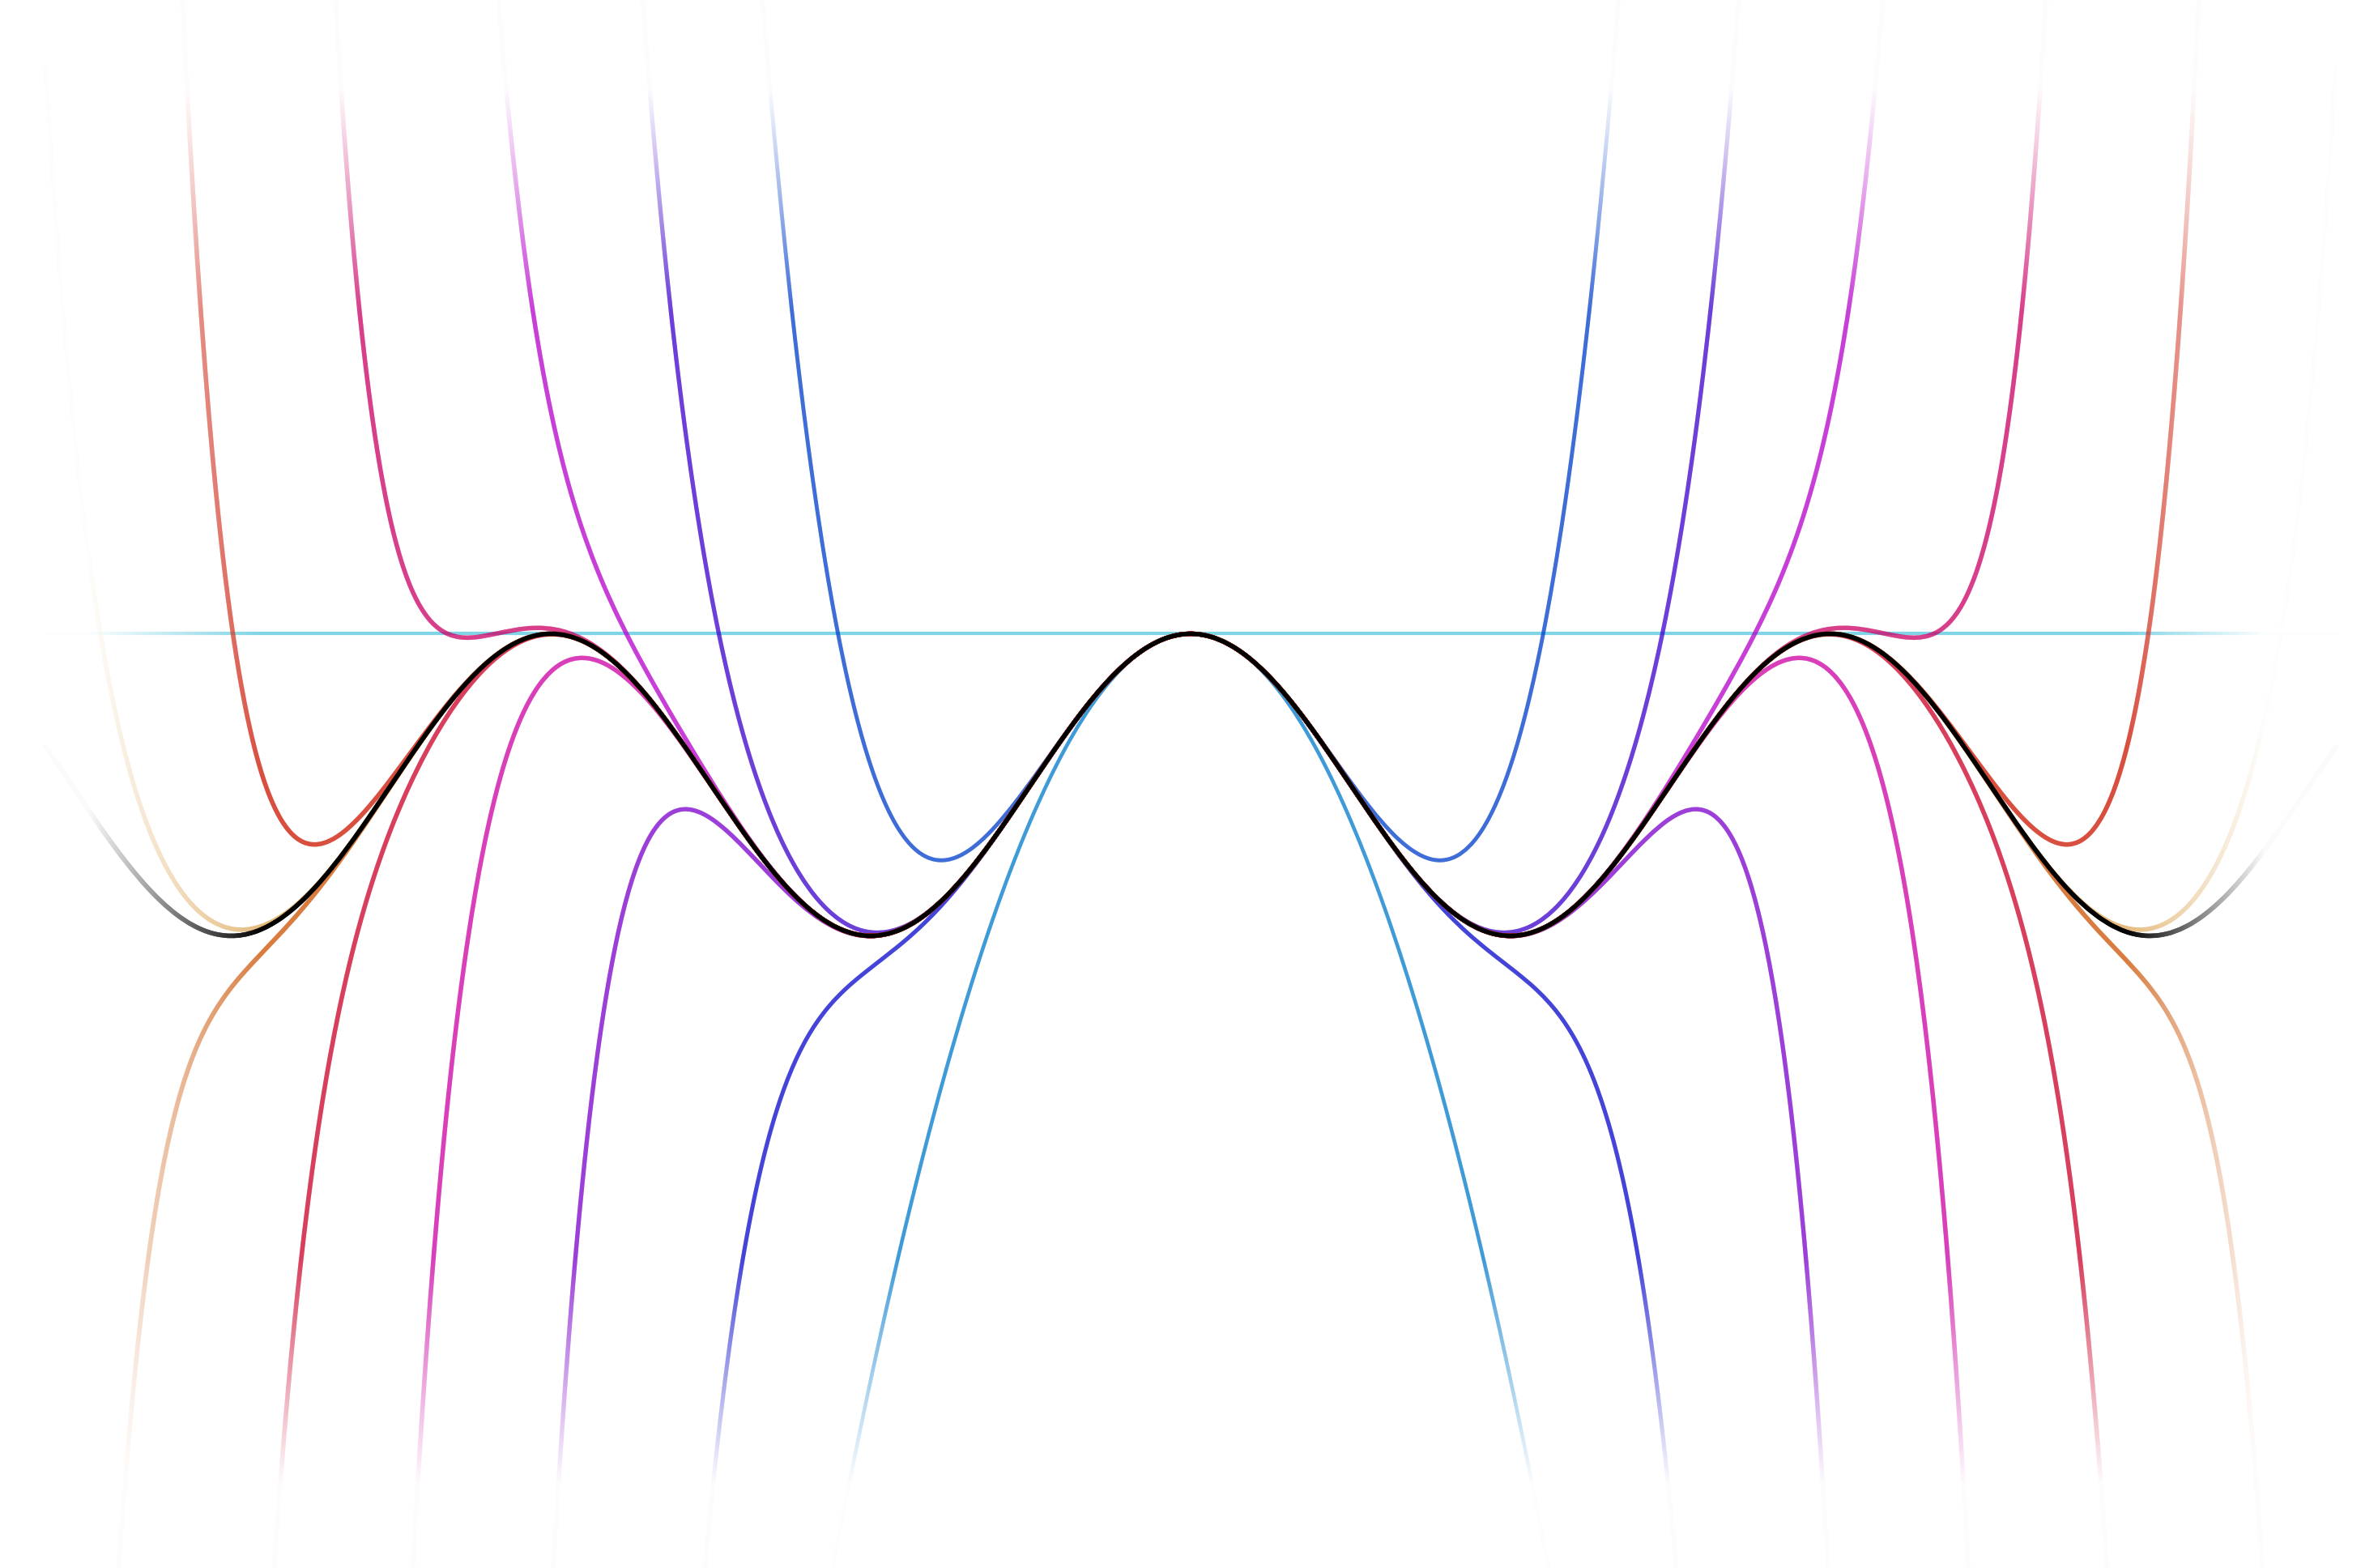
\includegraphics[width=\textwidth]{figures/forside3edit2.png} % also works with logo.pdf
   
    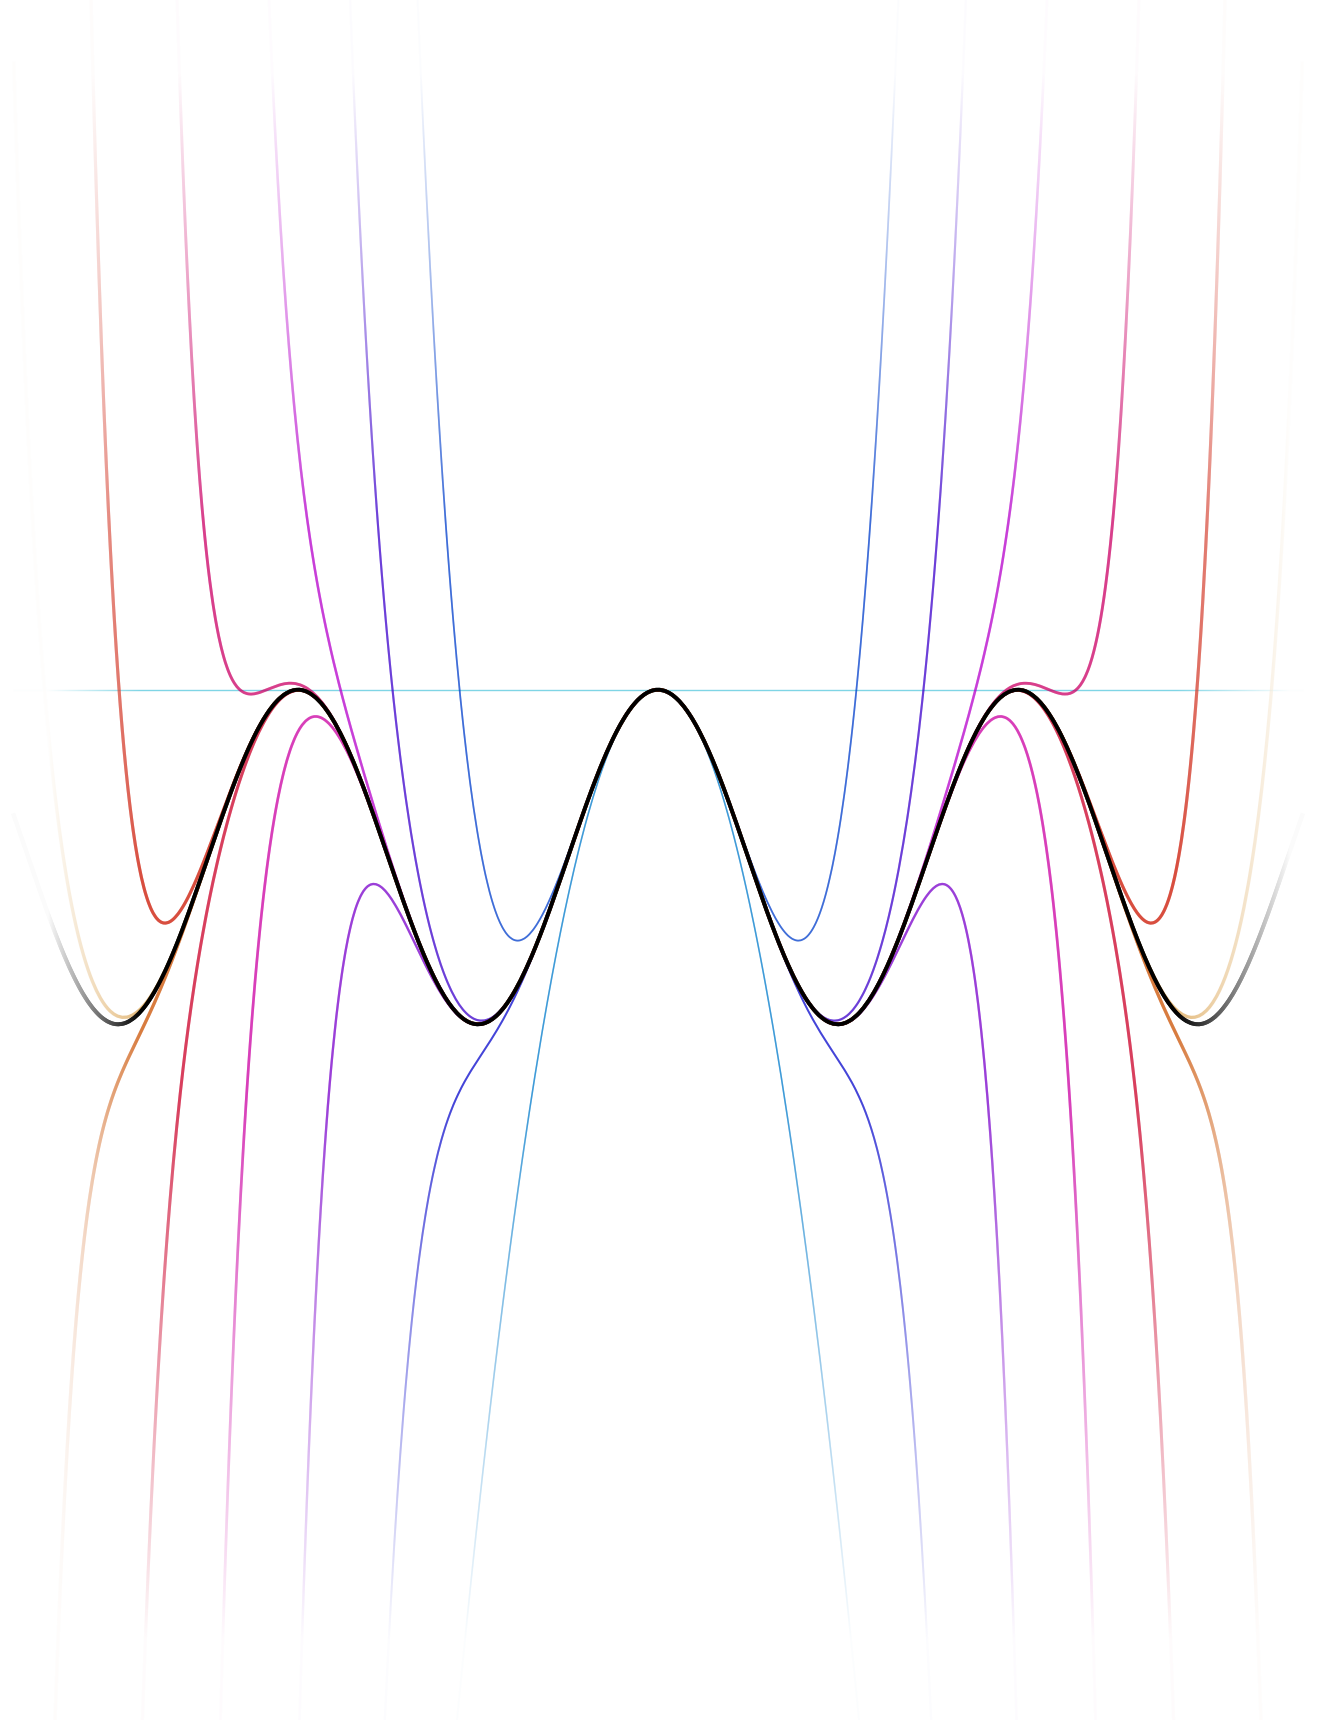
\includegraphics[width=\textwidth]{figures/forside4edit.png} % also works with logo.pdf
    \vfill
    \vfill
\thispagestyle{empty}

\end{titlepage}
%%%%% \footnote{hey} fyri vanligan footnote
%%%%%\footcite{talogrækker} fyri referencu
%%%%% :set spell spelllang=da (fyri at byrja spellcheck)
%%%% :set nospell fyri at sløkkja
%\setcounter{page}{2} % Set dette hvis første side tæller med i sidecount 
\section*{Resume} %150 ord (det essentielle i min opgave, dvs ca 8 linjer
\blindtext[1-2]
\tableofcontents
\newpage



\section{Indledning} %ca en halv side til en side. I egne ord, hvorfor dette er interessant. God ide at slutte af med problemformuleringen, "Og her vil jeg..."
Matematik kan synes firkantet og rigidt, hvor abstrakte forhold opskrives i eksakte formler, og hvor der ikke er plads til kreativitet. 
Dykker man dybere ind i faget vil man dog opdage, at dette ikke er tilfældet, og at der er mange situationer, hvor man gør kreativt brug af relativt ueksakte værktøjer. Et af disse er såkaldte Taylorpolynomier.


I matematikkens verden findes der alverdens slags funktioner, hvor nogle er mere medgørlige end andre. Nutidens computerteknik kræver eksempelvis hurtig og praktisk behandling af alle disse formler, og den forbindelse indtræder Taylorpolynomier ofte.\\
\\
Jeg vil i denne opgave beskrive den historiske baggrund for Taylorrækken. Jeg vil bevise formlen for Taylorrækken, undersøge dens restled, samt undersøge hvilke praktiske anvendelser Taylorpolynomier har i dag.

\section{Taylorrækkens historie} % Redegørelse Egne ord. Ikke inddrage citater (fordi så bliver det analyserende).
Matematikeren Brook Taylor (1685 - 1731) er navnefader til hvad vi i dag kalder Taylorpolynomier, efter at han i 1715 offentliggjorde en generel formel for principperne.
Taylors formel ser således ud i moderne form:\footcite[s. 247]{roy_2021}
\begin{equation}
   f(x)=f(a)+f(x-a)\frac{f'(a)}{1!}+(x-a)^2\frac{f''(a)}{2!}+\cdots. 
\end{equation}
Men Taylor var dog ikke den første der tænkte disse tanker.
\subsection{Newton}

Isaac Newton (1643 - 1727) opdagede disse samme principper femogtyve år tidligere end Taylor, uden at det blev udgivet.\footcite{roy_2021}\\
\\
\\
\\
\textcolor{blue}{Geometrien for et kompleks med et koordinationstal på 2 har en lineær rumlig struktur, mens et kompleks med et koordinationstal på 4 danner en tetraedisk eller plankvadratisk struktur, mens geometrien for et kompleks med et koordinationstal på 6 er oktaedisk. Et visuelt billede af den geometriske struktur for de nævnte koordinationstal fremgår af figur 1. Man skal huske, at disse modeller er idealiserede, og derfor kan geometrien afvige bl.a. pga. kvantemekaniske kræfter (Rossel, et. al. 1999, s. 203), (Rayner-Canham, et. al. 2006, s. 487).}

\textcolor{orange}{Sætningerne er formuleret i elevens egne ord, men med anvendelsen af præcise faglige begreber. Derudover inddrages figurer i form af fx tabeller, modeller og grafer, som anvendes aktivt i redegørelsen.
    De naturvidenskabelige fag vil ofte have et analytisk niveau som del af deres redegørelser, hvor opgaveformuleringen vil bede dig om at forklare bestemte sammenhænge eller karakterisere specifikke ting.}
\section{Analyse} % Kød og kartofler. Brug modellen (introducere citatet, så kommer citatet, og så kommenterer man.
\textcolor{orange}{Matematik er lidt anderledes, da matematik er et redskab til at kortlægge sammenhænge, fremfor at forklare dem. Det kan fx være at beskrive en lineær sammenhæng i en kemisk reaktion eller opstille en matematisk model for fx en udvikling i en smitsom sygdomsepidemi.  Du kan selvfølgelig også bruge matematikken i sig selv, hvor målet typisk vil være at bevise og illustrere matematiske sammenhænge.}
\section{Diskussion/Vurdering} % Måske tage nogle fagpersoner med eller noget. Gerne selv tage stilling.
\begin{equation}
    2+2=3
\end{equation}
\section{Konklusion} % samle problemformuleringens underspørgsmål. "jeg har. og så... jeg kan konkludere..."

\section{Litteraturliste}
%\nocite{*}
\subsection{Referenceliste}
\printbibliography
\subsection{Litteraturliste}
%\printbibliography[keyword=online]
Forsidebillede er skabt af undertegnede.
\end{document}

